%% Multi-Candidate Multimodal Advertisement Generation
%% IEEE conference format (IEEEtran). Compile: pdflatex x2 -> bibtex-free (manual refs)
\documentclass[conference]{IEEEtran}
\IEEEoverridecommandlockouts

\usepackage{cite}
\usepackage{amsmath,amssymb,amsfonts}
\usepackage{algorithmic}
\usepackage{graphicx}
\usepackage{textcomp}
\usepackage{xcolor}
\usepackage{booktabs}
\usepackage{multirow}
\usepackage{tikz}
\usetikzlibrary{arrows.meta,positioning,fit,backgrounds}
\def\BibTeX{{\rm B\kern-.05em{\sc i\kern-.025em b}\kern-.08em T\kern-.1667em\lower.7ex\hbox{E}\kern-.125emX}}

\setlength{\textfloatsep}{4pt plus 2pt minus 2pt}
\setlength{\floatsep}{3pt plus 2pt minus 2pt}
\setlength{\intextsep}{4pt plus 2pt minus 2pt}
\setlength{\abovecaptionskip}{3pt}
\setlength{\belowcaptionskip}{1pt}
\renewcommand{\arraystretch}{0.76}
\setlength{\abovedisplayskip}{4pt plus 2pt minus 2pt}
\setlength{\belowdisplayskip}{4pt plus 2pt minus 2pt}
\setlength{\abovedisplayshortskip}{2pt plus 2pt minus 1pt}
\setlength{\belowdisplayshortskip}{2pt plus 2pt minus 1pt}

\begin{document}

\title{Multi-Candidate Multimodal Advertisement Generation with
Learning-Based Performance Prediction and Intelligent Ranking}

\author{\IEEEauthorblockN{Mr. Alexander Aruldoss}
\IEEEauthorblockA{\textit{Faculty, Department of Information Science and Engineering} \\
\textit{Alva's Institute of Engineering and Technology, Mijar}\\
Mangalore, Karnataka, India \\
alexander.aruldoss@aiet.org.in}
\and
\IEEEauthorblockN{Disha}
\IEEEauthorblockA{\textit{Student, Department of Information Science and Engineering} \\
\textit{Alva's Institute of Engineering and Technology, Mijar}\\
Mangalore, Karnataka, India \\
dishagshetty6@gmail.com}
\and
\IEEEauthorblockN{Sanket}
\IEEEauthorblockA{\textit{Student, Department of Information Science and Engineering} \\
\textit{Alva's Institute of Engineering and Technology, Mijar}\\
Mangalore, Karnataka, India \\
biradarsanket380@gmail.com}
\and
\IEEEauthorblockN{Shankar C Akashkore}
\IEEEauthorblockA{\textit{Student, Department of Information Science and Engineering} \\
\textit{Alva's Institute of Engineering and Technology, Mijar}\\
Mangalore, Karnataka, India \\
shankarakashkore32@gmail.com}
\and[\break\hbox{}\hfill]
\IEEEauthorblockN{Sujal Bandekar}
\IEEEauthorblockA{\textit{Student, Department of Information Science and Engineering} \\
\textit{Alva's Institute of Engineering and Technology, Mijar}\\
Mangalore, Karnataka, India \\
sujalbandekar786@gmail.com}
}

\maketitle

\begin{abstract}
Generating advertising creative with diffusion models is cheap at the still-image
stage and expensive at the video stage. A single still costs roughly one-seventeenth
of a single eight-to-ten-second clip, so a job that animates every candidate spends
most of its budget on the last step. That shifts the useful question from \emph{how
good is one generated image} to \emph{which of several candidates is worth
animating}, a ranking problem that has to be answered one stage before any evidence
for it exists. We present a multi-candidate pipeline built around that problem.
Creative diversity is constructed geometrically instead of requested in words: a
Latin-hypercube draw over four categorical design axes yields $n$ candidate design
points whose minimum pairwise Hamming distance is provably maximal, so candidates
differ by construction and the construction can be ablated. Each design point is
compiled into a structured prompt and rendered by a latent diffusion backbone
conditioned on CLIP-family text embeddings and on reference images that carry model
and product identity. Surviving frames pass a quality gate of five pixel-level
measurements, whose thresholds are calibrated against a labelled render sweep
instead of being picked by hand. Each candidate is then represented by features from
frozen transformer and convolutional encoders, scored by a regression head trained
under a Bradley--Terry objective, and ranked by weighted composite score. Only the
promoted subset is animated and ranked again. We describe the architecture, survey
the diffusion, vision-language and preference-learning literature it builds on, and
state the implementation status as it stands. The sampler, brief compiler,
generation path, quality gate, feature extraction, ranking, delivery layer and
evaluation harness are implemented and exercised by 666 automated tests. The learned
prediction head still awaits the human preference corpus it must be trained on, so
the deployed scorer is a documented heuristic baseline, labelled as such wherever it
is displayed. We report the calibration measurements that exist, identify a
cross-validation leakage effect that inflates apparent accuracy by nineteen points
if left unguarded, and set out the evaluation protocol that remains to be run.
\end{abstract}

\begin{IEEEkeywords}
multimodal generation, latent diffusion, denoising diffusion probabilistic models,
CLIP, vision transformer, Bradley--Terry model, learning to rank, preference
learning, computational advertising, design-space sampling
\end{IEEEkeywords}

\section{Introduction}

Text-conditioned diffusion models have made a plausible advertising still routine to
produce, while a short advertising film is still expensive. That gap is the premise
of this work. In the pipeline described below, generating one candidate still takes
roughly two orders of magnitude less wall-clock time, and costs one order of
magnitude less in compute, than generating an eight-to-ten-second clip from it. A
job that generates five stills and animates all five therefore spends close to nine
tenths of its budget on animation, spread evenly over candidates that are not
equally good.

This puts the important decision at the boundary between the two stages: given
several candidate stills, which deserve to become video? The text-to-image
literature mostly asks a different question. It evaluates \emph{single-sample
fidelity} (does this image match this prompt, is it preferred, is it free of
artefacts) over independently sampled images
\cite{ho2020ddpm,rombach2022ldm,podell2023sdxl}. Advertising creative needs a
\emph{set} of candidates that covers the creative space, since a choice
between five near-duplicates is no choice, and a \emph{preference order} over that
set that is produced before the expensive stage instead of after it.

Both requirements are harder than they look. Diversity requested in natural language
(``give me five different concepts'') produces variation that cannot be measured,
reproduced under a fixed seed, or ablated. A preference order predicted at the still
stage is also a claim about the video stage, so showing that it is worth anything
takes paired observations at both stages and a protocol that does not compare the
system with itself.

We describe a system built around these two requirements and report its current
state, including what has not yet been done. The contributions are:

\begin{enumerate}
\item \textbf{Geometric design-space sampling.} A Latin-hypercube construction over
four categorical axes (camera angle, lighting, composition, motion intent)
guarantees the maximal minimum pairwise Hamming distance between candidates, so
diversity is a controlled quantity instead of a hoped-for property
(Section~\ref{sec:sampler}).
\item \textbf{A calibrated pre-ranking quality gate.} Five pixel-level checks, with
thresholds set on a labelled sweep of 150 lighting $\times$ composition $\times$
angle combinations, and a product-scale ceiling calibrated on real generations,
reject structurally broken frames before any ranking effort goes into them
(Section~\ref{sec:gate}).
\item \textbf{A frozen-encoder representation with an ablatable feature taxonomy.}
Nine disjoint feature groups (photometric, compositional, salience, palette,
contextual, embedding, aesthetic, identity and motion) are defined so that a group
can be removed \emph{exactly} and account for exactly one row of an ablation table
(Section~\ref{sec:features}).
\item \textbf{A two-stage ranking protocol with the confound stated.} The
image-stage ranking is committed to the record before any video exists, and a test
enforces that ordering. Model-to-model agreement between stages is reported as a
diagnostic, kept apart from the human-preference claim it could otherwise be
mistaken for (Sections~\ref{sec:rank} and~\ref{sec:threats}).
\end{enumerate}

Section~\ref{sec:lit} surveys the three literatures the work draws on.
Section~\ref{sec:method} describes the architecture module by module.
Section~\ref{sec:results} reports implementation status, the calibration
measurements so far, and the evaluation protocol still to be run.
Section~\ref{sec:conclusion} concludes.

\section{Literature Survey}
\label{sec:lit}

The relevant work falls into three strands: (i) conditional diffusion models for
image and video synthesis, (ii) frozen vision-language and vision encoders used as
general-purpose representations, and (iii) preference learning and ranking from
pairwise human judgements. Table~\ref{tab:lit} maps representative work in each
strand to the module of our architecture that uses it.

\subsection{Conditional Diffusion Synthesis}

Denoising diffusion probabilistic models \cite{ho2020ddpm} cast generation as the
reversal of a fixed Gaussian corruption process and introduced the noise-prediction
objective that our generation stage inherits. Song et al.\ \cite{song2021ddim} gave
a deterministic, non-Markovian sampler that needs far fewer function evaluations,
which made diffusion affordable inside an interactive pipeline. Rombach et al.\
\cite{rombach2022ldm} moved diffusion into the latent space of a pretrained
autoencoder, cutting the cost of high-resolution synthesis by roughly an order of
magnitude, and introduced the cross-attention mechanism that the brief compiler
writes into. Classifier-free guidance \cite{ho2022cfg} trades diversity against
conditioning fidelity at inference. Because our sampler produces diversity upstream,
strong guidance can be applied downstream without collapsing the candidate set.
Peebles and Xie \cite{peebles2023dit} replaced the convolutional U-Net with a
transformer, and Liu et al.\ \cite{liu2023rectflow} and Esser et al.\
\cite{esser2024sd3} reformulated the corruption path as a rectified flow. Our
generation stage targets that class of backbone, not one specific checkpoint. Ho et
al.\ \cite{ho2022vdm} extended diffusion to video, and Blattmann et al.\
\cite{blattmann2023svd} showed image-conditioned video diffusion, which is the
operation our animation stage applies to a promoted still. None of this work
supplies a selection criterion. Each paper evaluates samples, and none asks which of
several should be promoted to a more expensive downstream process. That gap is what
the prediction and ranking stages address.

\subsection{Frozen Encoders as Representations}

CLIP \cite{radford2021clip} showed that contrastive image-text pretraining at scale
yields an embedding that transfers well beyond its training task, and it supplied
the text encoder that conditions most later diffusion models. Zhai et al.\
\cite{zhai2023siglip} replaced CLIP's softmax contrastive loss with a pairwise
sigmoid loss, which improves quality at small batch sizes. SigLIP is the CLIP-family
encoder we use for the semantic feature block. DINOv2 \cite{oquab2023dinov2}
provides self-supervised visual features that keep fine-grained appearance detail,
where CLIP-family embeddings are weakest, and we use it for product-identity
similarity. ArcFace \cite{deng2019arcface} supplies the additive angular margin
embedding behind the face-identity check, which guards against drift from the
model's likeness. The LAION aesthetic predictor \cite{schuhmann2022laion}
contributes a single scalar, which we keep as its own ablation group instead of
folding it into the general embedding block. The annotation corpus holds hundreds of
comparisons, not millions, so all four encoders are frozen and only a small head is
fitted. Section~\ref{sec:prediction} quantifies that choice.

\subsection{Preference Learning and Ranking}

The Bradley--Terry model \cite{bradley1952} gives each item a scalar latent
strength, and the probability that one item beats another is a logistic function of
the difference in strengths. Hunter's minorization-maximization iteration
\cite{hunter2004mm} fits it and converges monotonically without a learning rate.
Burges et al.\ \cite{burges2005ranknet} showed that the same pairwise logistic
objective can sit on top of a parametric scorer, which turns ranking into supervised
learning on comparisons. Our prediction head adopts this formulation. ImageReward
\cite{xu2023imagereward}, PickScore \cite{kirstain2023pickapic} and Human Preference
Score \cite{wu2023hps} each fit a preference model on a large corpus of human
choices between generated images, and each shows that learned preference predicts
human judgement better than fidelity metrics such as FID or CLIP-score. These are
the closest antecedents to our work, but the target differs. All three rank images
to \emph{evaluate a generator}. Our system ranks candidates within a job to
\emph{allocate a downstream budget}, and its target variable is one modality removed
from the input. The class-imbalance and annotator-agreement problems those papers
document also apply to us, with greater force, because our corpus is smaller by
orders of magnitude.

\begin{table*}[t]
\caption{Summary of reviewed literature and relevance to the present system}
\label{tab:lit}
\centering
\tiny
\begin{tabular}{@{}p{2.7cm}p{2.3cm}p{5.0cm}p{5.4cm}@{}}
\toprule
\textbf{Author(s) / Year} & \textbf{Focus} & \textbf{Contribution} & \textbf{Relevance to this system} \\
\midrule
Ho et al.\ (2020) \cite{ho2020ddpm} & Diffusion generation & Introduced DDPM; generation as reversal of a fixed Gaussian corruption process, trained by noise prediction & Foundational basis for the generation stages \\
Song et al.\ (2021) \cite{song2021ddim} & Accelerated sampling & Deterministic non-Markovian sampler; order-of-magnitude fewer denoising steps & Keeps per-candidate generation cheap enough for a multi-candidate job \\
Rombach et al.\ (2022) \cite{rombach2022ldm} & Latent diffusion & Diffusion in autoencoder latent space with cross-attention text conditioning & Backbone architecture and conditioning path used here \\
Ho \& Salimans (2022) \cite{ho2022cfg} & Conditioning control & Classifier-free guidance; trades diversity for prompt fidelity at inference & High guidance is safe since diversity comes from the sampler \\
Peebles \& Xie (2023) \cite{peebles2023dit} & Denoiser architecture & Transformer denoiser replacing the convolutional U-Net & Backbone class the generation stage targets \\
Liu et al.\ (2023); Esser et al.\ (2024) \cite{liu2023rectflow,esser2024sd3} & Flow matching & Rectified-flow straight-line corruption paths; improved sample efficiency & Backbone-agnostic interface; current backbones combine this with DiT \\
Ho et al.\ (2022); Blattmann et al.\ (2023) \cite{ho2022vdm,blattmann2023svd} & Video diffusion & Spatiotemporal diffusion; image-conditioned video synthesis & The operation applied to a promoted still at animation \\
Radford et al.\ (2021) \cite{radford2021clip} & Vision-language pretraining & Contrastive image-text alignment; transferable joint embedding space & Text encoder conditioning generation and the semantic feature block \\
Zhai et al.\ (2023) \cite{zhai2023siglip} & Vision-language pretraining & Pairwise sigmoid loss removing batch-global normalisation & CLIP-family encoder used for the semantic embedding feature group \\
Oquab et al.\ (2023) \cite{oquab2023dinov2} & Self-supervised vision & Fine-grained visual features without language supervision & Product-identity similarity against the reference photograph \\
Deng et al.\ (2019) \cite{deng2019arcface} & Face representation & Additive angular margin loss for discriminative face embeddings & Face-identity check guarding against model-likeness drift \\
Schuhmann et al.\ (2022) \cite{schuhmann2022laion} & Aesthetic scoring & Linear aesthetic head over CLIP embeddings & Scalar aesthetic feature, isolated as its own ablation group \\
Bradley \& Terry (1952) \cite{bradley1952} & Paired comparison & Latent-strength model for pairwise outcomes & Objective for the prediction head and the ranking fit \\
Hunter (2004) \cite{hunter2004mm} & Estimation & MM iteration for Bradley--Terry; monotone convergence, no learning rate & Fitting procedure used for latent strengths \\
Burges et al.\ (2005) \cite{burges2005ranknet} & Learning to rank & Pairwise logistic objective over a parametric scorer & Formulation of the trainable prediction head \\
Xu et al.\ (2023); Kirstain et al.\ (2023); Wu et al.\ (2023) \cite{xu2023imagereward,kirstain2023pickapic,wu2023hps} & Generative preference & Learned human-preference models outperform FID/CLIP-score & Closest antecedents; this system ranks within a job, not across generators \\
\bottomrule
\end{tabular}
\end{table*}

\section{Implementation Methodology}
\label{sec:method}

The system is organised as nine sequential stages joined by an append-only job
record (Fig.~\ref{fig:arch}). Two properties of that record matter for the
architecture. First, each stage writes its output before the next stage reads it, so
the image-stage ranking is physically committed before any video exists, and an
automated test enforces that ordering. Second, every measurement carries an explicit
\emph{implemented} flag, so a check that has not been built reports that it is
missing instead of defaulting to a pass.

\begin{figure}[t]
\centering
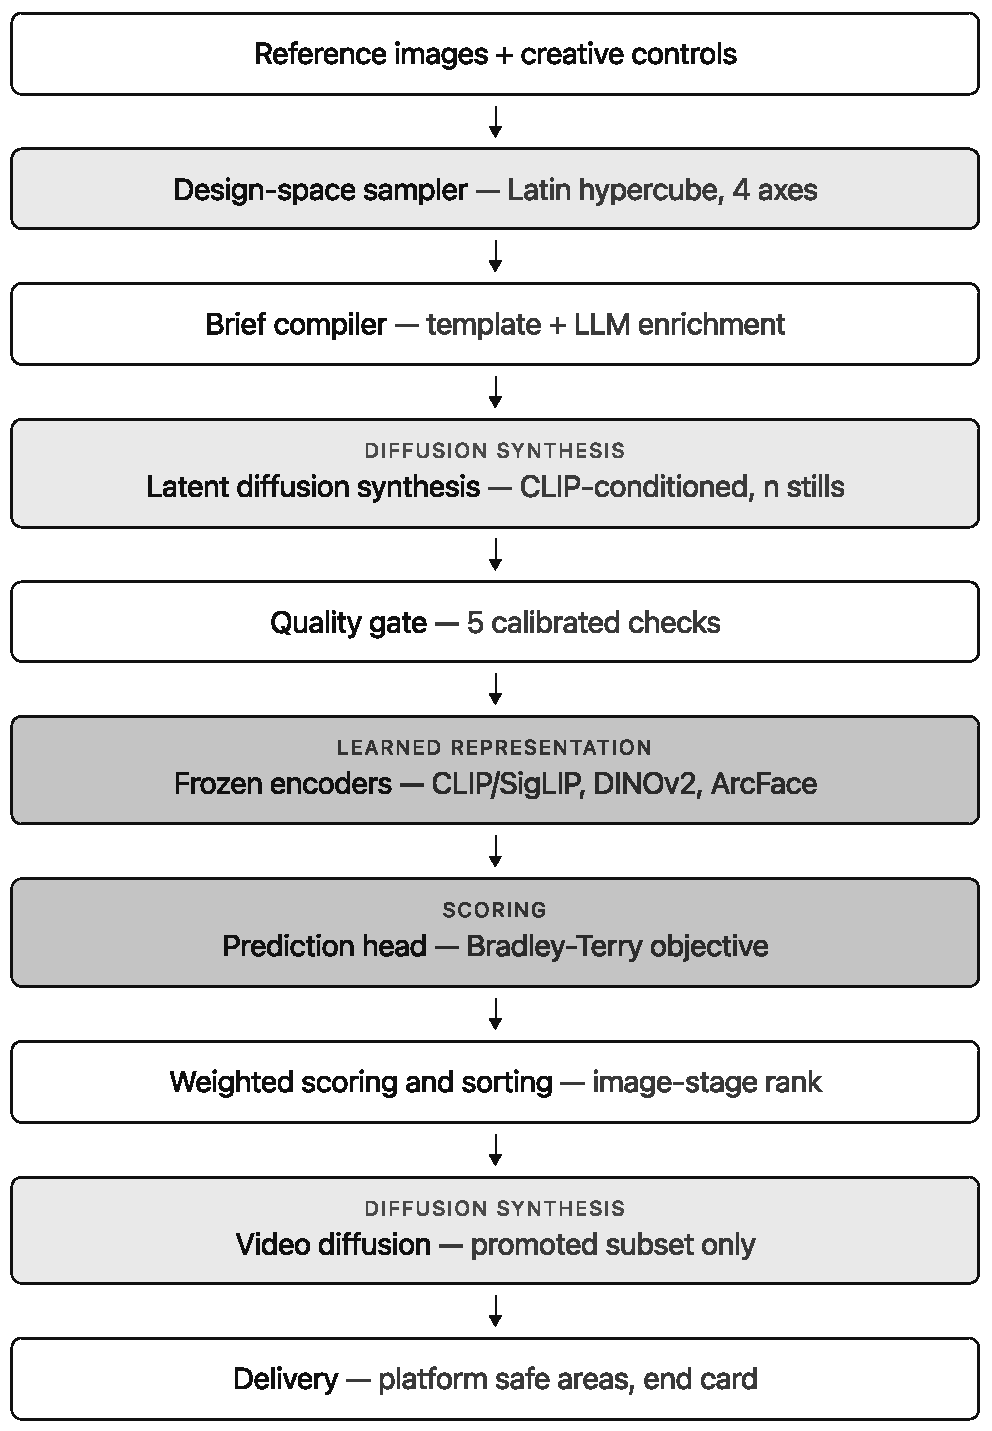
\includegraphics[width=0.68\columnwidth]{fig_architecture.pdf}
\caption{Pipeline architecture. Shaded stages are diffusion synthesis (light) and
learned representation and scoring (dark). The dashed boundary marks where the
ranking decides how the remaining budget is spent; only promoted candidates cross
it.}
\label{fig:arch}
\end{figure}

\subsection{Design-Space Sampling}
\label{sec:sampler}

We model the creative space as $A = 4$ categorical axes (camera angle, lighting,
composition and motion intent) with cardinalities $|L_a|$ for $a \in \{1,\dots,A\}$.
To produce $n$ candidates, the sampler draws a subset of $n$ \emph{distinct} levels
independently on each axis and pairs them positionally:

\begin{equation}
d_i = \big(\ell^{(1)}_{\pi_1(i)},\ \ell^{(2)}_{\pi_2(i)},\ \dots,\ \ell^{(A)}_{\pi_A(i)}\big),
\quad i = 1,\dots,n,
\label{eq:lhs}
\end{equation}

where $\pi_a$ is an independent permutation of the $n$ chosen levels on axis $a$.
Each axis contributes $n$ distinct levels and each candidate takes a different one,
so any two candidates differ on \emph{every} axis, which gives

\begin{equation}
\min_{i \neq j} \ \mathrm{Hamming}(d_i, d_j) \;=\; A
\qquad \text{whenever } n \le \min_a |L_a| .
\label{eq:hamming}
\end{equation}

This is the maximum attainable value, so there is nothing left to optimise; the
construction is optimal by definition, not by search. What \eqref{eq:hamming} buys
in practice is that diversity becomes an \emph{independent variable}. We can ablate
the sampler, either by replacing it with an unconstrained random draw or by
repeating a single design point, and measure the effect on downstream ranking
quality. That is impossible when diversity is delegated to a language model's sense
of variety.

\begin{figure}[t]
\centering
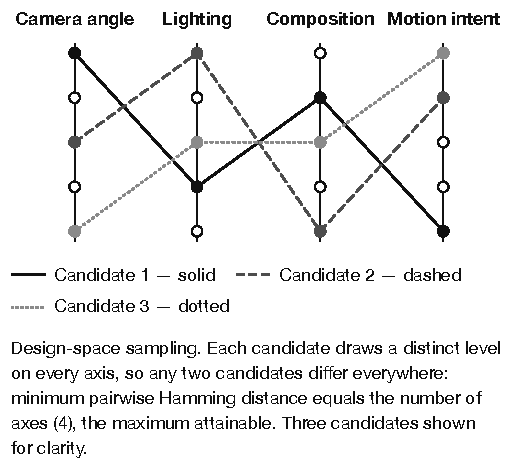
\includegraphics[width=0.68\columnwidth]{fig_design_space_sampling.pdf}
\caption{Three example candidates under the sampler of \eqref{eq:lhs}.}
\label{fig:sampling}
\end{figure}

Two mechanisms modulate the draw without breaking the guarantee. A \emph{mood}
parameter reweights which levels are preferred on each axis; if the preferred pool
cannot supply $n$ distinct values, the draw widens to the full axis instead of
duplicating a level. A user-locked camera angle collapses that axis to a constant
and lowers the bound in \eqref{eq:hamming} to $A-1=3$. The sampler reports the
reduced distance instead of hiding it.

The sampler also applies one structural exclusion. The \texttt{negative\_space\_top}
composition places the subject low in the frame to leave room for overlaid text. On
vertical placements that puts the subject beneath platform chrome, which covers the
bottom $18$ to $22\%$ of the frame. The measured safe-area saliency share for this
composition is $0.44$ to $0.67$, against $0.68$ to $0.91$ for every other
composition, so it fails the gate structurally and not just occasionally. We exclude
it in the sampler because otherwise we would pay to generate a candidate that is
guaranteed to be rejected.

\subsection{Brief Compilation}

A template compiles each design point into a generation prompt and writes the
structural constraints out explicitly: the positional roles of the reference images,
the camera angle and lighting phrases, the composition, the brand palette and the
safe-area requirement. Naming the references by position, meaning which input
carries the model's likeness and which carries the product, is the most effective
intervention against identity drift. It is also exactly the material that a language
model asked to be creative will paraphrase away.

For that reason a language model enriches \emph{only} the free-form scene
description and a one-line concept, and the structural section never passes through
it. If the language model is unavailable or returns malformed output, the template
result stands alone and the job proceeds. This fallback is not an exceptional path:
every offline test run takes it, so it is exercised continuously.

\subsection{Conditional Image Synthesis}

Generation follows the standard latent diffusion formulation
\cite{ho2020ddpm,rombach2022ldm}. An encoder maps an image to a latent
$z_0$; a forward process adds Gaussian noise over $T$ steps according to a variance
schedule $\{\beta_t\}$,

\begin{equation}
q(z_t \mid z_{t-1}) = \mathcal{N}\!\left(z_t; \sqrt{1-\beta_t}\, z_{t-1},\ \beta_t \mathbf{I}\right),
\label{eq:forward}
\end{equation}

which admits the closed form $z_t = \sqrt{\bar\alpha_t}\, z_0 + \sqrt{1-\bar\alpha_t}\,\epsilon$
with $\bar\alpha_t = \prod_{s\le t}(1-\beta_s)$ and $\epsilon \sim \mathcal{N}(0,\mathbf{I})$.
A denoiser $\epsilon_\theta$ is trained to invert it under the conditioning signal
$c$:

\begin{equation}
\mathcal{L} = \mathbb{E}_{z_0,\, \epsilon,\, t}
\Big[\big\lVert \epsilon - \epsilon_\theta(z_t,\, t,\, c) \big\rVert_2^2 \Big].
\label{eq:objective}
\end{equation}

The conditioning signal $c$ has two components. The first is text: the compiled
brief, embedded by a CLIP-family transformer encoder
\cite{radford2021clip,zhai2023siglip} and injected through cross-attention. The
second is the pair of reference images, which carry model and product appearance
through the backbone's image-conditioning path. This second component makes the task
editing and composition instead of free synthesis, and it is why identity
preservation can be measured at all. At inference, classifier-free guidance
\cite{ho2022cfg} combines conditional and unconditional predictions,

\begin{equation}
\tilde\epsilon_\theta(z_t, t, c) = \epsilon_\theta(z_t, t, \varnothing)
+ w\big(\epsilon_\theta(z_t, t, c) - \epsilon_\theta(z_t, t, \varnothing)\big),
\label{eq:cfg}
\end{equation}

with guidance weight $w$. Sampling uses a deterministic solver \cite{song2021ddim}
and each candidate carries a fixed seed, so a job is reproducible: the same design
point, brief and seed yield the same latent trajectory. The research design requires
this, because the sampler ablation of \eqref{eq:lhs} can only be interpreted if the
downstream generation step is held constant.

\subsection{Quality Gate}
\label{sec:gate}

Five pixel-level measurements screen candidates before any ranking effort is spent
on them. We fitted the thresholds with a calibration sweep over 150 lighting
$\times$ composition $\times$ angle combinations, rendered with matched and
deliberately mismatched brand palettes. Each threshold sits \emph{below the observed
minimum} of the legitimate class instead of at its median, because a filter that
rejects a third of usable candidates costs more than it saves. Table~\ref{tab:gate}
lists the measured ranges and the thresholds chosen.

\begin{table}[t]
\caption{Quality-gate checks, measured on-brand ranges, and thresholds}
\label{tab:gate}
\centering
\tiny
\begin{tabular}{@{}p{1.85cm}p{1.5cm}p{1.35cm}p{2.1cm}@{}}
\toprule
\textbf{Check} & \textbf{On-brand range} & \textbf{Threshold} & \textbf{Catches} \\
\midrule
Palette adherence & 0.912--0.972 (off-brand 0.000) & $\ge 0.456$ & Brand-colour violation \\
Safe-area saliency & 0.680--0.914 & $\ge 0.55$ & Subject under platform chrome \\
Focal clarity & 0.578--0.728 & $\ge 0.25$ & Smeared attention, no subject \\
Luminance & 0.531--0.643 & $[0.06, 0.96]$ & Black or blown frames \\
Contrast & 0.180--0.248 & $\ge 0.03$ & Flat or empty frames \\
Product area share & see Sec.~\ref{sec:gate} & $\le 0.16$ & Product larger than the person \\
\bottomrule
\end{tabular}
\end{table}

The product-area check is the only one with a ceiling instead of a floor, and the
only threshold calibrated on real generations instead of the synthetic sweep. We
added it because early live jobs rendered the product far larger than the person
holding it, a failure that none of the existing checks expressed. Focal clarity over
the same eleven frames spans $0.31$ to $0.50$, with correct and oversized frames
interleaved, so it separates nothing. Product area share does:

\begin{center}
\footnotesize
\begin{tabular}{@{}lll@{}}
visibly correct scale & $0.011$--$0.094$ & ($n=5$) \\
unlabelled & $0.084$--$0.113$ & ($n=3$) \\
visibly oversized & $0.172$--$0.294$ & ($n=3$) \\
\end{tabular}
\end{center}

\noindent The classes separate with a gap of $0.059$. The threshold sits near the
top of that gap, for the same asymmetry as above: a false reject costs a paid
regeneration, while a miss only lets one more frame into ranking. Eleven frames make
a calibration set and not a validation set, and the code flags this as the first
threshold due for revision as the corpus grows.

Two further checks compare face and product identity against the reference images.
They compute a real cosine similarity, using ArcFace and DINOv2 respectively,
whenever an embedding archive is available, but they still report
\texttt{implemented = false} unconditionally. No calibration sweep has measured
where same- and different-identity pairs separate for this generator, so any
threshold we set now would be invented and not calibrated. The measured value is
still surfaced and propagated as \emph{pending}, so no interface can present it as a
verified pass. The missing piece is not the computation, which is tested end to end,
but the fact that nothing in the synchronous request path can run a GPU encoder
inline.

\subsection{Representation}
\label{sec:features}

Each surviving candidate is represented by a feature vector assembled from nine
disjoint groups (Table~\ref{tab:groups}). The partition is the unit of ablation, so
it has to be exact: a group must be removable without residue, because an ablation
that leaves a correlated proxy behind reports a contribution that is not there.

\begin{table}[t]
\caption{Feature groups and their provenance}
\label{tab:groups}
\centering
\tiny
\begin{tabular}{@{}p{1.6cm}p{4.1cm}p{1.5cm}@{}}
\toprule
\textbf{Group} & \textbf{Content} & \textbf{Source} \\
\midrule
Photometric & Exposure, contrast, saturation & Pixels \\
Composition & Position and extent of the salient mass & Pixels \\
Salience & Saliency concentration, safe-area compliance & Pixels \\
Palette & Brand-palette adherence & Pixels \\
Context & The sampler's design coordinate, vertical, platform & Job record \\
Embedding & Reduced CLIP/SigLIP and DINOv2 blocks & Frozen encoder \\
Aesthetic & LAION aesthetic score & Frozen encoder \\
Identity & DINOv2 product and ArcFace face similarity to references & Frozen encoder \\
Motion & Motion energy, temporal consistency, hook strength & Video only \\
\bottomrule
\end{tabular}
\end{table}

Ablating the \emph{context} group answers a research question directly. The group
contains only the design coordinate the sampler chose, so removing it tests whether
the creative decision carries information independent of how the render turned out.

The frozen encoders run as a separate offline stage that writes a compressed
embedding archive, which the trainable head consumes. The head is implemented once
and used by both the evaluation harness and the serving path, so the model reported
in an ablation table is bit-identical to the model the system scores with. There is
no train/serve reimplementation gap that could make the reported numbers wrong.

This stage guards against silent zero-filling. An item without an embedding must not
receive a zero vector, because after standardisation a zero vector \emph{is} the
feature-space mean and would look average instead of missing. Coverage is returned
alongside the matrix, and uncovered items are dropped explicitly. Deterministic
pseudo-embeddings also exist so the training path can be exercised without running
the encoders. A synthetic flag propagates into the evaluation output, so any table
built on them says so.

\subsection{Performance Prediction}
\label{sec:prediction}

The prediction head is a parametric scorer $s_\theta$ over the feature vector
$\phi(x)$, trained directly on pairwise comparisons under the Bradley--Terry
likelihood \cite{bradley1952,burges2005ranknet}. For a comparison in which
candidate $i$ was preferred to candidate $j$,

\begin{equation}
\Pr(i \succ j) = \sigma\big(s_\theta(\phi(x_i)) - s_\theta(\phi(x_j))\big),
\qquad \sigma(u) = \frac{1}{1+e^{-u}},
\label{eq:bt}
\end{equation}

and the head is fitted by minimising the regularised negative log-likelihood over
the observed comparison set $\mathcal{C}$:

\begin{equation}
\mathcal{L}(\theta) = -\!\!\sum_{(i,j)\in\mathcal{C}}\!\! w_{ij}\,
\log \sigma\big(s_\theta(\phi(x_i)) - s_\theta(\phi(x_j))\big)
\;+\; \lambda \lVert \theta \rVert_2^2 .
\label{eq:loss}
\end{equation}

Ties are kept and enter as two half-weight observations in opposing directions.
Discarding them would remove the observations where candidates are close, which is
where a ranker's behaviour matters most.

\textbf{The number of labels, not the encoders, sets model capacity.} The default
head is linear. With approximately $1{,}200$ training comparisons, a defensible
parameter budget is on the order of $80$, while a single eight-unit hidden layer
over thirty inputs already needs roughly $250$. We implemented a hidden-layer
variant so the report can \emph{show} what exceeding that budget does. It gets one
table row and is explicitly not the headline model.

When latent strengths are estimated from comparisons alone, as when ranking without
features, the Bradley--Terry model is fitted with Hunter's minorization-maximization
iteration \cite{hunter2004mm}. It converges monotonically and needs no learning
rate, autograd or GPU. Under plain MM, an item that wins every comparison it appears
in has unbounded strength. A phantom-opponent prior, meaning a few games credited
against a fixed-strength opponent with half won and half lost, keeps the estimates
finite and pulls sparsely observed items toward the centre.

We also implemented an alternative two-step formulation that fits strengths first
and then regresses features onto them. The theoretical objection is that squared
error over-weights the least-observed, most-extreme strengths. That did not appear
in our simulations: the two-step fit stayed within a point of the direct fit over
simulated corpora of 25 to 200 sets. The pairwise objective remains primary anyway,
because it needs no intermediate fit and treats ties as observations.

\subsection{Ranking and Promotion}
\label{sec:rank}

Candidate scores are combined into a composite by weighted scoring and sorting.
For candidate $i$ with component scores $c_{ik}$ and weights $w_k$ summing to one,

\begin{equation}
S_i = \sum_{k} w_k\, c_{ik},
\qquad
\text{rank}(i) = \big|\{\, j : S_j > S_i \,\}\big| + 1 ,
\label{eq:weighted}
\end{equation}

with ties broken deterministically by identifier. The top-$m$ candidates by $S_i$
are promoted. The rest stay in the record with their scores and gate measurements,
so a job documents what it declined to animate and why. The image-stage ranking is
written to the record \emph{before} any video generation is dispatched. The research
claim depends on this ordering, and a test enforces it instead of relying on
developer discipline.

After the promoted candidates are animated, the finished videos are ranked again
over a feature set extended by the motion group. The quantity of interest is the
agreement between the two orderings, measured by Spearman's rank correlation

\begin{equation}
\rho = 1 - \frac{6 \sum_{i=1}^{m} d_i^2}{m\,(m^2-1)},
\qquad d_i = r^{\text{img}}_i - r^{\text{vid}}_i ,
\label{eq:spearman}
\end{equation}

together with pairwise agreement accuracy and bootstrap intervals, since a point
estimate over a few hundred comparisons is not a result. Each job contributes one
paired observation, so the evaluation dataset grows as the system is used. We report
the cost consequence as a counterfactual: had only the top-ranked still been
animated, how often would the human-preferred video have been retained? This
quantifies the saving without the system having had to make the cut.
Section~\ref{sec:threats} describes the confound that limits how \eqref{eq:spearman}
can be interpreted at present.

\subsection{Video Synthesis and Delivery}

An image-conditioned video diffusion model \cite{ho2022vdm,blattmann2023svd}
animates each promoted still into a clip of eight to ten seconds, with the motion
intent from \eqref{eq:lhs} supplying camera and subject motion. A composited end
card carrying the brand mark and web address is appended within the clip's declared
duration at no additional cost. Delivery renders each clip for seven placement
targets across four aspect ratios and applies the same platform safe-area inset that
the gate's saliency check was calibrated against.

\subsection{Technology Stack}
\label{sec:stack}

The orchestration API is Python/FastAPI on top of an SQLAlchemy-backed relational
store that holds the append-only job records, the spend ledger and the annotation
corpus. Pipeline stages, feature extraction, ranking and evaluation are written in
NumPy with no deep-learning framework dependency, which keeps the trained head
identical across evaluation and serving. The frozen encoders run in a separate GPU
environment and communicate through a compressed embedding archive. The operator
interface is TypeScript/Next.js. Its client-side types are generated from the Python
schema by a drift-checked generator, so the two halves cannot disagree about a job's
shape.

\section{Result and Analysis}
\label{sec:results}

The system is a mid-development prototype and not a deployed product. This section
reports its status and does not present evaluation figures that have not yet been
produced.

\subsection{Implementation Status}
\label{sec:implstatus}

The design-space sampler, brief compiler, conditional generation path, quality gate,
feature extraction, ranking, video animation, multi-platform delivery, spend ledger
and evaluation harness are implemented and exercised end to end. The 666 automated
tests include ones that enforce the research-critical invariants: the image-stage
ranking is committed before video generation, pending gate checks cannot present as
passing measurements, and a replayed job collapses onto the job it replays instead
of counting as a second observation.

The learned prediction head is implemented, together with its training script,
cross-validation protocol, baseline comparisons and per-group ablation. It has not
been trained on real human preference labels, because the annotation corpus does not
exist yet. \textbf{The scorer currently deployed is therefore a documented,
hand-weighted heuristic baseline, and every interface that displays one of its
scores flags it as a placeholder.} Three conditions mark a score as a placeholder: a
model trained on stand-in embeddings, a model whose held-out accuracy was never
measured, and a model measured at chance. The face- and product-identity gate checks
now compute a real cosine similarity against an embedding archive when one is
supplied (Section~\ref{sec:gate}), and tests exercise this against synthetic
archives. On a live job today no archive is supplied, so both checks still report as
pending, and their thresholds await the same kind of calibration sweep that every
other check in Table~\ref{tab:gate} required. No trained-model accuracy figure
exists, and we do not claim one.

\subsection{Experimental Setup}
\label{sec:setup}

The measurements below were not produced by a benchmark harness against a trained
model, since none exists yet. This subsection therefore says what was run to produce
every number here and in Section~\ref{sec:threats}. Three independent calibration
protocols underlie them. They share no data with one another, and none touches the
still-untrained prediction head. The gate's five pixel-level thresholds
(Table~\ref{tab:gate}) were fitted against 150 lighting $\times$ composition
$\times$ angle combinations rendered with matched and deliberately mismatched brand
palettes. The product-area ceiling was calibrated separately, against eleven
hand-labelled frames from two real, paid jobs, because the synthetic sweep does not
reproduce the failure it targets. The cross-validation leakage measurement
(Section~\ref{sec:threats}) used 60 synthetic generation sets whose features were
constructed to be uninformative. True pairwise accuracy on them is therefore chance,
and any deviation from chance comes from the split and not from signal in the
features. This isolates the leakage mechanism from the separate, still-open question
of whether real features carry signal.

\subsection{Preliminary Observations}

The measurements that exist are calibration measurements, reported in
Section~\ref{sec:method} and summarised here. The gate's five primary thresholds
were fitted against a 150-combination render sweep in which the on-brand and
off-brand palette classes separate with a gap of $0.912$ (Table~\ref{tab:gate},
Fig.~\ref{fig:gatecal}). By construction, each threshold sits below the legitimate
class's observed minimum. The product-area ceiling was calibrated against eleven
frames from real generations, where the correctly scaled and oversized classes
separate with a gap of $0.059$ while focal clarity fails to separate them at all
(Fig.~\ref{fig:productarea}). The compositional exclusion in the sampler was
measured in the same way: $0.44$ to $0.67$ safe-area saliency share, against $0.68$
to $0.91$ for the alternatives.

\begin{figure}[t]
\centering
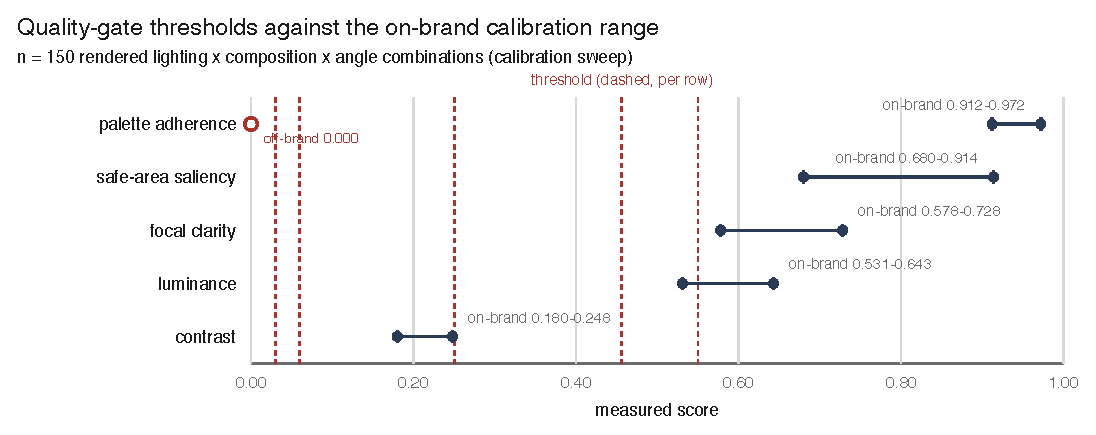
\includegraphics[width=0.62\columnwidth]{fig_gate_calibration.pdf}
\caption{The five quality-gate thresholds of Table~\ref{tab:gate} against their
calibration ranges. Every threshold sits below its class's observed minimum. The
palette check's off-brand point is shown hollow for contrast.}
\label{fig:gatecal}
\end{figure}

\begin{figure}[t]
\centering
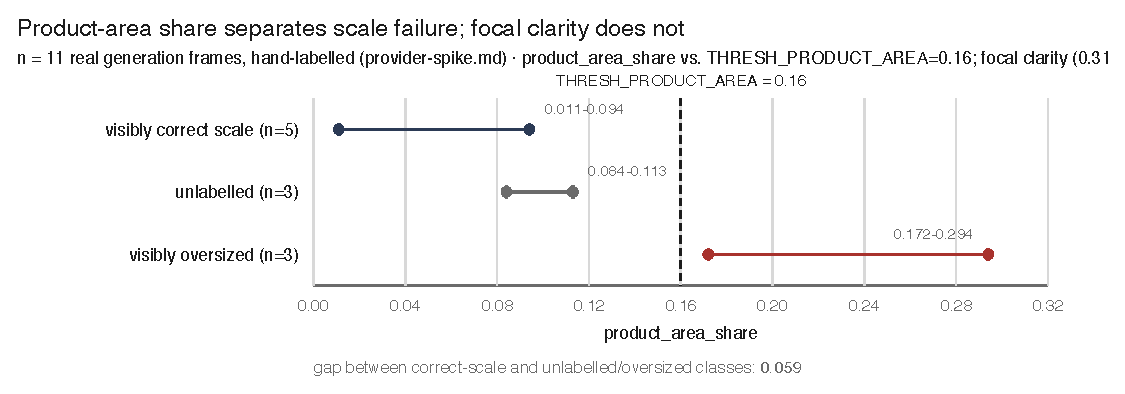
\includegraphics[width=0.62\columnwidth]{fig_product_area_separation.pdf}
\caption{Product-area share separates the three labelled classes with a $0.059$ gap.
Focal clarity, measured over the same eleven frames, spans $0.31$ to $0.50$ with
correct and oversized frames interleaved, so it cannot.}
\label{fig:productarea}
\end{figure}

On a representative completed job, the cost split matched the prediction in
Section~I. The five candidate stills were generated and gated for approximately
$15\%$ of the job total, and the two promoted candidates took the remaining $85\%$
at animation (Fig.~\ref{fig:costsplit}). This is a spend measurement and not a
quality one, and it confirms that the budget is concentrated where the ranking
decision sits. The unit prices are fixed provider prices, not estimates: a still
costs \$0.04 and a ten-second clip \$0.70, a ratio of $17.5\times$ that matches the
``one-seventeenth'' figure in Section~I. The default job of five stills and two
promoted videos therefore costs \$1.60, against a \$35.00 total budget tracked by
the same ledger. Animating every candidate would cost \$3.70 for the same five
stills, which is the cost the ranking stage exists to avoid.

\begin{figure}[t]
\centering
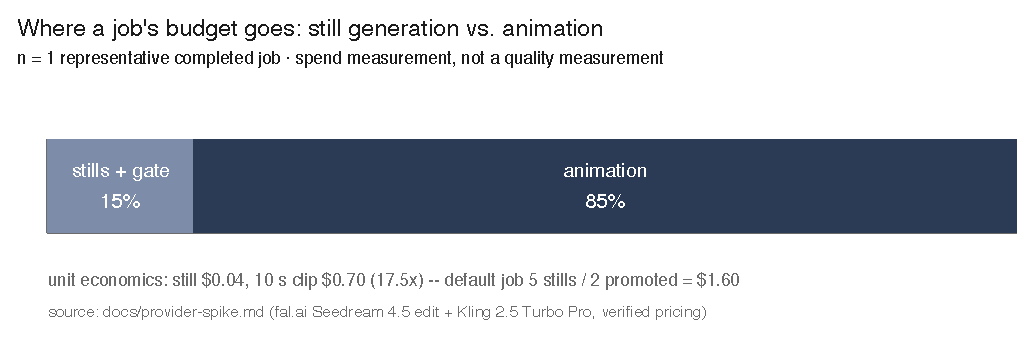
\includegraphics[width=0.62\columnwidth]{fig_cost_split.pdf}
\caption{Spend split for a representative job, with the unit prices behind it. Video
is $17.5\times$ the price of a still, so promoting two of five instead of animating
all five is the difference between \$1.60 and \$3.70.}
\label{fig:costsplit}
\end{figure}

Figure~\ref{fig:qualitative} shows the actual candidates from one completed job
(\$1.60, five stills, two promoted) instead of a schematic. It gives the image-stage
order that the ranking committed to the record, each candidate's heuristic-baseline
placeholder score, and which two were promoted. The video stage reordered the
promoted pair: the image stage predicted B\,\textgreater\,C, and the finished videos
ranked C\,\textgreater\,B. This is a concrete instance of the confound that
Section~\ref{sec:threats} states in the abstract. An image-stage prediction is a
claim about the video stage, and this job is one observation of that claim being
tested. It has not yet been validated against human judgement.

\begin{figure*}[t]
\centering
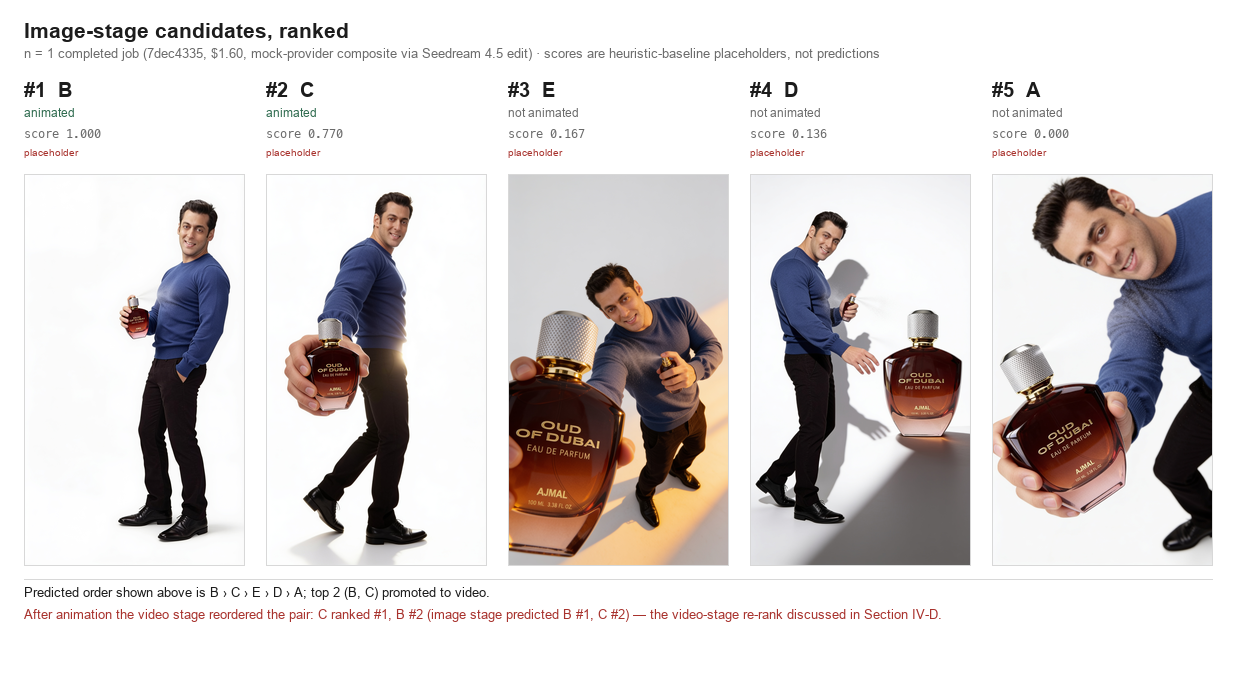
\includegraphics[width=0.44\textwidth]{fig_qualitative_ranking.png}
\caption{Image-stage candidates from a real completed job (id \texttt{7dec4335},
product ``Perfume'', \$1.60), in the order the ranking committed to the record.
Scores are the heuristic baseline described in Section~\ref{sec:implstatus}, not a
trained prediction. After animation, the video stage ranked C above B, reversing
the image-stage order shown here for the promoted pair.}
\label{fig:qualitative}
\end{figure*}

\subsection{Threats to Validity}
\label{sec:threats}

We identified three methodological hazards during construction. Each can produce a
result that looks plausible but is fictional.

\textbf{Cross-validation leakage across generation sets.} Comparisons from the same
generation set share candidates, so a split randomised over \emph{comparisons} puts
near-duplicate observations on both sides of the fold boundary. On features that are
uninformative by construction, so that true accuracy is chance, a comparison-level
split reports $0.659$ pairwise accuracy and a set-level split reports $0.465$
(Fig.~\ref{fig:leakage}). The choice of split alone accounts for nineteen points of
accuracy that are not real. We therefore always cross-validate over generation sets
and never over comparisons.

\begin{figure}[t]
\centering
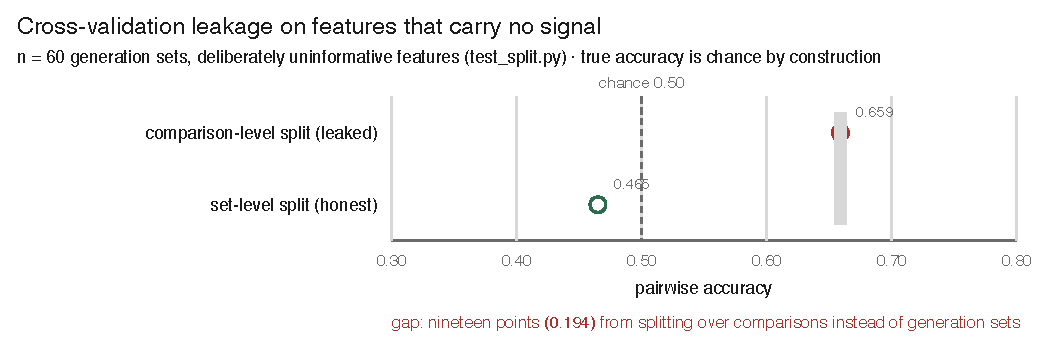
\includegraphics[width=0.50\columnwidth]{fig_cv_leakage.pdf}
\caption{The leakage effect on features built to carry no signal. Splitting over
comparisons instead of generation sets produces nineteen points of accuracy that are
not real.}
\label{fig:leakage}
\end{figure}

\textbf{Model-to-model agreement is not the research claim.} The claim is that
image-stage prediction anticipates how people prefer finished \emph{videos}. Both
stages are scored by the same codebase over overlapping feature groups, so some
agreement is guaranteed by construction, and \eqref{eq:spearman} computed today
measures internal consistency and not predictive validity. We therefore report
agreement as a diagnostic and report the human comparison as \emph{absent} until
video-stage judgements exist. Quoting the first as the second would be the most
likely way for this project to overclaim.

\textbf{Replay inflation.} Deterministic replay of a stored job writes a fresh
record with a new identifier and bit-identical candidates. If observations were
counted by job identifier, a replay script run twenty times would report twenty sets
in perfect agreement, with a zero-width confidence interval. That would be a
fabricated headline result from code that looks correct. Sets are therefore keyed by
a hash of their candidates' content digests, so a replayed job collapses onto the
job it replays. If two records share a set key but disagree in order, that is scorer
nondeterminism, and it is surfaced as a defect and not averaged away.

\subsection{Limitations and Planned Evaluation}
\label{sec:limitations}

The central limitation of this paper is that five results a reader would expect are
not yet available. We name them here so that nobody has to infer them from their
absence: a trained-model performance figure, a human preference dataset, baseline
comparison results, per-group ablation results, and human video-preference
validation. All five depend on the same missing input, the pairwise human preference
corpus described in Section~\ref{sec:prediction}, which does not exist yet. None of
them is approximated, simulated or estimated from proxy data here, because that
would produce the kind of plausible but fictional result that
Section~\ref{sec:threats} guards against. The deployed scorer is therefore a
documented heuristic baseline throughout, and it is never presented as a trained
model.

Once the corpus exists, we will run the following protocol: (i) collect pairwise
preference judgements over image-stage candidates and, separately, over the finished
videos, with enough overlap to estimate inter-annotator agreement; (ii) establish
the accuracy ceiling that a perfect predictor could reach against single noisy
judgements, and report accuracy as a fraction of it; (iii) evaluate the trained head
against random, aesthetic-only and gate-score-only baselines as \emph{paired}
comparisons with bootstrap intervals; (iv) run the per-group ablation of
Table~\ref{tab:groups} against the full model, paying particular attention to the
context group; (v) report the image-to-video rank agreement of \eqref{eq:spearman}
against human judgements, together with the promotion counterfactual; and (vi)
ablate the sampler of \eqref{eq:lhs} against an unconstrained draw. A confidence
interval wider than the gaps between models is itself the finding.

\section{Conclusion}
\label{sec:conclusion}

This paper presented a multi-candidate multimodal advertisement generation pipeline
built around a cost asymmetry. Still-image synthesis is cheap and video synthesis is
not, so the decision that matters is which candidates to animate, and it has to be
made one stage before the evidence for it exists. The system addresses this with a
Latin-hypercube design-space sampler whose diversity guarantee is provable and
ablatable; a latent diffusion generation stage conditioned on CLIP-family text
embeddings and identity-carrying reference images; a quality gate whose thresholds
are calibrated on labelled render sweeps and not picked by hand; a frozen-encoder
representation partitioned into exactly ablatable feature groups; and a
Bradley--Terry-trained prediction head that feeds a weighted scoring and sorting
stage, which commits its ranking to the record before any video exists.

As Section~\ref{sec:results} reports, the generation, gating, representation,
ranking, animation, delivery and evaluation infrastructure is implemented and
covered by 666 automated tests. The learned prediction head still awaits its human
preference corpus, and the deployed scorer remains a documented heuristic baseline
that is marked as a placeholder wherever it appears. We claim no trained-model
performance figure. The immediate next steps are to collect the pairwise annotation
corpus, run the evaluation protocol of Section~\ref{sec:results}, and calibrate the
two pending identity checks. Longer term, the image-stage predictor should be
retrained continuously on the paired observations that the system accumulates in
normal operation. That is what lets the ranking claim be tested at increasing scale
instead of just once.

\scriptsize
\setlength{\itemsep}{0pt}
\setlength{\parskip}{0pt}
\begin{thebibliography}{00}

\bibitem{ho2020ddpm} J. Ho, A. Jain, and P. Abbeel, ``Denoising diffusion probabilistic models,'' in \emph{Adv. Neural Inf. Process. Syst. (NeurIPS)}, vol. 33, 2020, pp. 6840--6851.

\bibitem{song2021ddim} J. Song, C. Meng, and S. Ermon, ``Denoising diffusion implicit models,'' in \emph{Proc. Int. Conf. Learn. Representations (ICLR)}, 2021.

\bibitem{rombach2022ldm} R. Rombach, A. Blattmann, D. Lorenz, P. Esser, and B. Ommer, ``High-resolution image synthesis with latent diffusion models,'' in \emph{Proc. IEEE/CVF Conf. Comput. Vis. Pattern Recognit. (CVPR)}, 2022, pp. 10684--10695.

\bibitem{ho2022cfg} J. Ho and T. Salimans, ``Classifier-free diffusion guidance,'' \emph{arXiv:2207.12598}, 2022.

\bibitem{peebles2023dit} W. Peebles and S. Xie, ``Scalable diffusion models with transformers,'' in \emph{Proc. IEEE/CVF Int. Conf. Comput. Vis. (ICCV)}, 2023, pp. 4195--4205.

\bibitem{liu2023rectflow} X. Liu, C. Gong, and Q. Liu, ``Flow straight and fast: Learning to generate and transfer data with rectified flow,'' in \emph{Proc. Int. Conf. Learn. Representations (ICLR)}, 2023.

\bibitem{esser2024sd3} P. Esser \emph{et al.}, ``Scaling rectified flow transformers for high-resolution image synthesis,'' in \emph{Proc. Int. Conf. Mach. Learn. (ICML)}, 2024.

\bibitem{podell2023sdxl} D. Podell \emph{et al.}, ``SDXL: Improving latent diffusion models for high-resolution image synthesis,'' in \emph{Proc. Int. Conf. Learn. Representations (ICLR)}, 2024.

\bibitem{ho2022vdm} J. Ho, T. Salimans, A. Gritsenko, W. Chan, M. Norouzi, and D. J. Fleet, ``Video diffusion models,'' in \emph{Adv. Neural Inf. Process. Syst. (NeurIPS)}, 2022.

\bibitem{blattmann2023svd} A. Blattmann \emph{et al.}, ``Stable video diffusion: Scaling latent video diffusion models to large datasets,'' \emph{arXiv:2311.15127}, 2023.

\bibitem{radford2021clip} A. Radford \emph{et al.}, ``Learning transferable visual models from natural language supervision,'' in \emph{Proc. Int. Conf. Mach. Learn. (ICML)}, 2021, pp. 8748--8763.

\bibitem{zhai2023siglip} X. Zhai, B. Mustafa, A. Kolesnikov, and L. Beyer, ``Sigmoid loss for language image pre-training,'' in \emph{Proc. IEEE/CVF Int. Conf. Comput. Vis. (ICCV)}, 2023, pp. 11975--11986.

\bibitem{oquab2023dinov2} M. Oquab \emph{et al.}, ``DINOv2: Learning robust visual features without supervision,'' \emph{Trans. Mach. Learn. Res. (TMLR)}, 2024.

\bibitem{deng2019arcface} J. Deng, J. Guo, N. Xue, and S. Zafeiriou, ``ArcFace: Additive angular margin loss for deep face recognition,'' in \emph{Proc. IEEE/CVF Conf. Comput. Vis. Pattern Recognit. (CVPR)}, 2019, pp. 4690--4699.

\bibitem{schuhmann2022laion} C. Schuhmann \emph{et al.}, ``LAION-5B: An open large-scale dataset for training next generation image-text models,'' in \emph{Adv. Neural Inf. Process. Syst. (NeurIPS) Datasets and Benchmarks}, 2022.

\bibitem{bradley1952} R. A. Bradley and M. E. Terry, ``Rank analysis of incomplete block designs: I. The method of paired comparisons,'' \emph{Biometrika}, vol. 39, no. 3/4, pp. 324--345, 1952.

\bibitem{hunter2004mm} D. R. Hunter, ``MM algorithms for generalized Bradley--Terry models,'' \emph{Ann. Statist.}, vol. 32, no. 1, pp. 384--406, 2004.

\bibitem{burges2005ranknet} C. Burges \emph{et al.}, ``Learning to rank using gradient descent,'' in \emph{Proc. Int. Conf. Mach. Learn. (ICML)}, 2005, pp. 89--96.

\bibitem{xu2023imagereward} J. Xu \emph{et al.}, ``ImageReward: Learning and evaluating human preferences for text-to-image generation,'' in \emph{Adv. Neural Inf. Process. Syst. (NeurIPS)}, 2023.

\bibitem{kirstain2023pickapic} Y. Kirstain, A. Polyak, U. Singer, S. Matiana, J. Penna, and O. Levy, ``Pick-a-Pic: An open dataset of user preferences for text-to-image generation,'' in \emph{Adv. Neural Inf. Process. Syst. (NeurIPS)}, 2023.

\bibitem{wu2023hps} X. Wu \emph{et al.}, ``Human preference score: Better aligning text-to-image models with human preference,'' in \emph{Proc. IEEE/CVF Int. Conf. Comput. Vis. (ICCV)}, 2023.

\end{thebibliography}

\end{document}
